\scanpage{50}
\[
\deleted{\Pi_p(B_1,\mathbin{-},B_n)=\sum_{J\in\unsure{\mathcal P}_p[1,n]}}
\qquad B_i=B'_i+4
\]
\deleted{$\unsure{\Sigma}$}
\[
B'_1B'_2=B'_2B'_3=\mathbin{--}=B'_nB'_{n-1}=0
\]
\[
(2-\tfrac{B_1}{2})(2-\tfrac{B_2}{2})\cdots(2-\tfrac{B_n}{2})
=\frac{(-1)^n}{2^n}.
\]
\[
L_1=2\qquad L'_1=1
\]
\[
L_2=4-B_1\deleted{\unsure{+B_2}}
=\deleted{\unsure{4-(\alpha_0+\alpha_1)-\alpha_0+}}
2-\alpha_0=-(\alpha_0-2)
\]
\[
L_3=8-2(B_1+B_2\deleted{\unsure{+B_3}})
=-2[\alpha_1+\alpha_2+\deleted{\unsure{\alpha_0+\alpha_1}}]
\]
\[
L_4=\underbrace{16-4(B_1+B_2+B_3+\deleted{\unsure{B_4}})
+\left(\sum_{1\leq i\leq j\leq3}B_iB_j\right)}
-(B_1B_2+B_2B_3+B_3B_4)
\]
\[
\deleted{(2-\tfrac{B_1}{2})(2-\tfrac{B_2}{2})}
\]
\[
\begin{aligned}
&-4(\alpha_1+\alpha_2+\alpha_3+\deleted{\unsure{\alpha_4}})-8\\
&\quad+\bigl[
\deleted{(\alpha_0+2)(\alpha_1+2)}
+(\alpha_0+2)(\alpha_2+2)
+\deleted{\unsure{(\alpha_1+2)(\alpha_3+2)}}\\
&\hspace{8em}+\deleted{\unsure{(\alpha_2+2)(\alpha_3+2)}}\bigr]
\end{aligned}
\]
\[
\deleted{\begin{aligned}
=&-4-4(\alpha_0+\alpha_1+\alpha_2\deleted{\unsure{+\alpha_3}})
+2(\alpha_0+\alpha_1+\alpha_2+\alpha_3+\alpha_2+\alpha_3)\\
&+\alpha_0\alpha_2+\alpha_0\alpha_3
\end{aligned}}
+\alpha_1\alpha_3
\]
\[
\deleted{\unsure{2\alpha_0+2\alpha_1+2\alpha_2+2\alpha_3}}
\]
\[
\begin{aligned}
&=-4-2(\alpha_1+\inserted{2\alpha_2+}\alpha_3)
+(\alpha_1\alpha_3\deleted{\unsure{+\alpha_0\alpha_3+\alpha_2\alpha_3}})\\
&=(\alpha_1-2)(\alpha_3-2)\unsure{-}4(\alpha_2+2)
\end{aligned}
\]
\figure{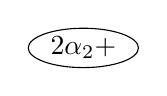
\begin{tikzpicture}
\draw (0,0) ellipse (.7 and .25);\node at (0,0){$2\alpha_2+$};
\end{tikzpicture}}
\uline{NB}\quad
$L_{n-1}(B_1,\mathbin{-},B_{n-1})
=L_{n-1}(B_{n-1},\ldots,B_1)$
\figure{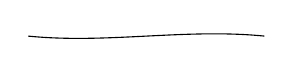
\begin{tikzpicture}\draw (0,0)..controls(1,-.1)and(2,.1)..(3,0);\end{tikzpicture}}
\[
\begin{aligned}
&\det\left(
\begin{array}{cccccc}
2\deleted{\unsure{C_{-1}}}&-C_0&0&&&\\
-C_0&2C_0&-C_1&0&&\\
0&-C_1&2C_1&&&0\\
0&0&-C_2&\ddots&C_{n-2}&-C_{n-1}\\
&--&&0&-C_{n-1}&2C_{n-1}
\end{array}\right)\\
&=\Delta_{n+1}(\underbrace{1,C_0,\mathbin{-},C_{n-1}}_{n+1\ \text{arg.}})
=2\Delta_n(C_0,\mathbin{-},C_{n-1})
-C_0^2\Delta_{n-1}(C_1,\mathbin{-},C_{n-1})
\end{aligned}
\]
\inserted{\deleted{\unsure{n+1}}\quad ordre $n+1$}
\[
=\delta_{n+1}(1,B_0,\ldots,B_{n-1})
=B_0^nB_1^{n-1}\mathbin{-}B_{n-1}
L_{n+1}(\deleted{\unsure{1}}B_0,\mathbin{-},B_{n-1})
\]
\[
\deleted{L_2(1,B_0)=4-}
\]
\[
\deleted{\unsure{\tfrac12\delta_{n+1}(1,B_0,\ldots,B_{n-1})}}
\qquad
\deleted{L_3(\unsure{1},B_0,}
\]
\[
\delta_2(1,B_0)\deleted{\unsure{B_1}}
=B_0L_2(1,B_0)=B_0(4-B_0)
=-(\alpha_0+2)(\alpha_0-2)=4-\alpha_0^2
\]
\[
\delta'_3(1,B_0,B_1)
=B_0^2B_1L'_3(\deleted{\unsure{1}}B_0,B_1)
=\deleted{\unsure{B_0^2B_1}}\deleted{\unsure{2}}
-B_0^2B_1(\alpha_0+\alpha_1)
\]
\[
\delta_4(1,B_0,B_1,B_2)
=B_0^3B_1^2B_2
\underbrace{L_4(B_0,B_1,B_2)}_{(\alpha_0-2)(\alpha_2-2)-4(\alpha_1+2)}
\]
\margin{\[
\deleted{\begin{aligned}
\det\begin{pmatrix}2C_0&-C_1\\-C_1&2C_1\end{pmatrix}
&=4C_0C_1-C_1^2\\
&=C_1(4C_0-C_1)\\
&=B_0^2B_1(4-B_1)
\end{aligned}}
\]}
\mspage{49}

